%
% gerade.tex
%
% (c) 2018 Prof Dr Andreas Müller, Hochschule Rapperswil
%
\section{Geraden%
\label{skript:section:geraden}}
\rhead{Geraden}
Die affine Geometrie definiert Geraden und Ebenen als die primären Objekte
sowie Schnittpunkte und Schnittgerade und mithin die Parallelität als die
zentralen Eigenschaften, mit denen die Geometrie aufgebaut werden soll.
Es ist daher höchste Zeit, dass wir auch für Geraden und Ebenen eine
vektorielle Beschreibung finden und das Finden von Schnittpunkten
und Schnittgeraden auf rechnerische Art ermöglichen.

%
% Geraden in der Ebene und im Raum
%
\subsection{Geraden in der Ebene und im Raum}
Die erste Beschreibung einer Geraden mit Hilfe von Koordinaten, die man in
der Schule normalerweise kennenlernt, die des Graphs einer Funktion
$y=ax+b$.
Diese Beschreibung hat aber mindestens zwei Schwächen, die sie für eine
weiterführende Theorie ungeeignet macht.
\begin{enumerate}
\item Sie funktioniert nur in der Ebene und lässt sich nicht auf die
dreidimensionale Situation verallgemeinern.
\item Vertikale Geraden lassen sich damit nicht beschreiben.
Damit wird die Vertikale zu einer speziellen Richtung, so etwas darf
es in der affinen Geometrie nicht geben.
\end{enumerate}
Wir sind daher gezwungen, eine verallgemeinerungsfähigere und symmetrischere
Beschreibung einer Geraden zu finden.

Parallele Geraden haben alle die gleiche Richtung, sie enthalten alle
den gleichen Vektor.
Ausgehend von einem Punkt ausserhalb einer gegebenen Geraden kann eine
parallele Gerade konstruiert werden.
Eine Gerade kann also beschrieben werden durch einen Punkt und einen
Richtunsgvektor.
Im Vektorbild müssen wir die Menge der Punkte der Geraden $g$ durch ihre
Ortsvektoren beschreiben.
Sei also $P_0$ der Ausgangspunkt der Geraden und $P$ ein beliebiger
Punkt.
Der Vektor von $P_0$ nach $P$ muss daher ein Vielfaches des
{\em Richtungsvektors} $\vec{r}$ sein:
\[
\overrightarrow{P_0P} = t\vec{r}.
\]
Der Ortsvektor $\vec{p}$ von $P$ erfüllt daher die Gleicung
\begin{equation}
\vec{p} = \vec{p}_0 + t\vec{r}.
\label{skript:punktrichtung}
\end{equation}
Dies ist die {\em Parameterdarstellung} der Geraden, manchmal auch die
{\em Punkt-Richtungs-Form} der Geradengleichung genannt.
Der Ortsvektor $\vec{p}_0$ des Ausgangspunktes $P_0$ heisst auch
{\em Stützvektor}.

Wir überprüfen, dass diese Form der Geradengleichung tatsächlich die
oben genannten Unzulänglichkeiten nicht hat:
\begin{enumerate}
\item Tatsächlich haben wir in der Herleitung der
Parameterdarstellung~\eqref{skript:punktrichtung} keine Voraussetzungen
darüber gemacht, ob die Vektoren zwei- oder dreidimensional sind.
\item Die vertikalen Geraden in der Ebenen können zum Beispiel durch die
Parameterdarstellung
\[
\{ (x_0,y)\;|\; y\in\mathbb R\}
=
\left\{
\left.
\begin{pmatrix}x_0\\0\end{pmatrix}
+
y\begin{pmatrix}0\\1\end{pmatrix}
\;
\right|
\;
y\in\mathbb R
\right\}
\]
beschrieben werden.
\end{enumerate}

\subsubsection{Geschwindigkeit}
Interpretiert man $t$ als die Zeit, dann bewegt sich ein Punkt auf der
Geraden mit der Parameterdarstellung
\[
\vec{p} = \vec{p}_0 + t \vec{v}
\]
ausgehend vom Punkt $P_0$ in einer Sekunde um $\vec v$,
dieser Vektor stellt also die Geschwindigkeit des Punktes dar.
Die Parameterdarstellung der Geraden ist also auch eine
Beschreibung einer gleichförmigen Bewegung mit {\em Geschwindigkeitsvektor}
$\vec{v}$.

\subsubsection{Gerade durch zwei Punkte}
\begin{aufgabe}
Gegeben zwei Punkte $A$ und $B$, finde die Parameterdarstellung einer
Geraden durch die beiden Punkte.
\end{aufgabe}
\begin{proof}[Lösung]
Als Stützvektor kann der Ortsvektor von $A$ verwendet werden, als Richtung
der Vektor von $A$ nach $B$:
\[
\vec{p}
=
\overrightarrow{OA} + t\overrightarrow{AB}
=
\vec{a} + t(\vec{b}-\vec{a})
\]
Allerdings kann genauso gut auch $\vec{b}$ als Stützvektor verwendet
werden und $\vec{a}-\vec{b}$ als Richtungsvektor.
\end{proof}

\begin{beispiel}
Man finde die Parameterdarstellung der Geraden durch die Punkte
$A=(3,1,4)$ und $B=(1,5,9)$.

\smallskip

{\parindent 0pt
Dazu} braucht man einen Vektor, der die Funktion von $\vec p$ übernehmen
kann, wir verwenden $\vec{a}$ dafür, und als
Richtungsvektor können wir $\vec{b}-\vec{a}$ verwenden.
Damit wird die Geradengleichung
\begin{equation}
\vec r(t) =
\begin{pmatrix}3\\1\\4 \end{pmatrix}
+t
\begin{pmatrix}-2\\4\\5\end{pmatrix}.
\label{pigerade}
\end{equation}
Wir werden diese Gerade in nachfolgenden Beispielen weiter verwenden.
\end{beispiel}


\subsubsection{Liegt ein Punkt auf einer Geraden?}
Gegeben ist die Gerade durch $\vec p$ mit Richtungsvektor $\vec v$.
Geht die
Gerade durch den Punkt $\vec s$? Offenbar müssen wir herausfinden, ob es
einen Wert des Parameters $t$ gibt, für den der Geradenpunkt mit $\vec s$
identisch ist, also
\[
\vec s = \vec p + t\vec v.
\]
Diese Vektorgleichung ist genau genommen ein Gleichungssystem für die einzelnen
Komponenten
\[
\begin{pmatrix}
s_1\\s_2\\s_3
\end{pmatrix}
=
\begin{pmatrix}
p_1\\p_2\\p_3
\end{pmatrix}
+t
\begin{pmatrix}
v_1\\v_2\\v_3
\end{pmatrix}
\qquad
\Rightarrow
\qquad
\begin{aligned}
s_1&=p_1+tv_1\\
s_2&=p_2+tv_2\\
s_3&=p_3+tv_3
\end{aligned}
\]
Dieses Gleichungssystem mit drei Gleichungen aber nur einer Unbekannten $t$
wird meistens nicht lösbar sein.
Aber es gilt natürlich die übliche Alternative
für lineare Gleichungssysteme:
\begin{itemize}
\item Es kann keine Lösungen geben: Dieser Fall tritt ein, wenn die Gerade
an dem Punkt vorbei geht.
\item Es kann unendlich viele Lösungen geben: Dieser Fall tritt ein, wenn
$\vec v=0$ ist und $\vec p=\vec s$.
Dann ``bleibt'' der Punkt $\vec r(t)$
immer am Ort $\vec p$, welcher identisch ist mit dem gesuchten Punkt $\vec s$.
\item Es kann genau eine Lösung geben: falls $\vec v\ne 0$ und der Punkt auf der
Geraden liegt, gibt es genau einen Parameterwert, für den der Punkt
getroffen wird.
\end{itemize}
Den Parameterwert im Fall 3 kann man zum Beispiel finden, indem man eine
der Gleichungen auswählt, in der der $v_i$-Koeffizient nicht $0$ ist
Diese Gleichung löst man nach $t$ auf.
Falls $v_1\ne 0$ heisst das
\[
t=\frac{s_1-p_1}{v_1}.
\]
Durch Einsetzen in die anderen Gleichungen kann man anschliessend auch überprüfen,
ob die Gerade tatsächlich durch den Punkt geht.

\begin{beispiel} Welcher der Punkte $U=(5,-3,-1)$ und $V=(7,-7,-7)$
liegt auf der Geraden (\ref{pigerade})?

\smallskip

{\parindent 0pt Um zu testen},
ob die Gerade durch den Punkt mit Ortsvektor $\vec u$
geht, muss man versuchen, die Gleichung
\[
\begin{pmatrix}3\\1\\4 \end{pmatrix}
+t
\begin{pmatrix}-2\\4\\5\end{pmatrix}
=\vec u
\]
zu lösen.
Für die beiden Ortsvektoren $\vec u$ und $\vec v$
bedeutet das
\begin{align*}
\begin{pmatrix}3\\1\\4 \end{pmatrix}
+
t_1
\begin{pmatrix}-2\\4\\5\end{pmatrix}
&=
\begin{pmatrix}5\\-3\\-1\end{pmatrix}
&
\qquad
\begin{pmatrix}3\\1\\4 \end{pmatrix}
+
t_2
\begin{pmatrix}-2\\4\\5\end{pmatrix}
&=
\begin{pmatrix}7\\-7\\-7\end{pmatrix}
\\
t_1
\begin{pmatrix}-2\\4\\5\end{pmatrix}
&=
\begin{pmatrix}5\\-3\\-1\end{pmatrix}
-
\begin{pmatrix}3\\1\\4 \end{pmatrix}
=
\begin{pmatrix}2\\-4\\-5 \end{pmatrix}
&
\qquad
t_2
\begin{pmatrix}-2\\4\\5\end{pmatrix}
&=
\begin{pmatrix}7\\-7\\-7\end{pmatrix}
-
\begin{pmatrix}3\\1\\4 \end{pmatrix}
=
\begin{pmatrix}4\\-8\\-11\end{pmatrix}
\\
t_1&=-1,&t_2&:\text{keine Lösung.}
\end{align*}
Es folgt, dass $U$ auf der Geraden liegt, $V$ aber nicht.
\end{beispiel}


%
% Schnittpunkte
%
\subsection{Schnittpunkte}

\begin{aufgabe}
Gegeben zwei Geraden $g_1$ und $g_2$ mit Parameterdarstellungen
\[
\vec{r} = \vec{p} + t\vec{r}
\qquad\text{und}\qquad
\vec{r} = \vec{q} + t\vec{v},
\]
finde ihren Schnittpunkt.
\end{aufgabe}

\begin{proof}[Lösungen]
Man beachte, dass in dieser Aufgabe $t$ ein Platzhalter ist, dass also
der Schnittpunkt zu verschiedenen Werten in jeder Parameterdarstellung
erreicht wird.
Wir müssen also zwei Variablen $t$ und $s$ bestimmen, so dass die beiden
Parameterdarstellungen den gleichen Punkt ergeben.
Wir müssen also die Gleichung
\[
\vec{p} + t\vec{r}
=
\vec{q} + s\vec{v}
\]
nach $t$ und $s$ auflösen.
Indem man die Vektorgleichung in Komponenten schreibt
\begin{align*}
p_1+tr_1 &= q_1+sv_1\\
p_2+tr_2 &= q_2+sv_2\\
p_3+tr_3 &= q_3+sv_3
\end{align*}
und die Unbekannten $\color{red}t$ und $\color{red}s$ auf die linke Seite bringt, erhält
man ein lineares Gleichungssystem 
\begin{align*}
r_1{\color{red}t}-v_1{\color{red}s}&= q_1-p_1\\
r_2{\color{red}t}-v_2{\color{red}s}&= q_2-p_2\\
r_3{\color{red}t}-v_3{\color{red}s}&= q_3-p_3.
\end{align*}
Dies ist ein Gleichungssystem mit zwei Unbekannten, für die Anzahl der Lösungen
gilt wieder die bekannte Alternative:
\begin{itemize}
\item Keine Lösungen: Die Geraden haben keinen Schnittpunkt, in der Ebene
kann dies zum Beispiel dadurch geschehen, dass die Geraden parallel sind.
Im Raum können die Geraden auch windschief sein.
In drei Dimensionen erhalten wir drei Gleichungen mit nur einer Unbekannten,
dieses System wir normalerweise nicht lösbar sein.
\item Unendlich viele Lösungen: die Geraden sind deckungsgleich
\item Genau eine Lösung: es gibt einen wohldefinierten Schnittpunkt.
\end{itemize}
Gelöst werden kann das Gleichungssystem natürlich mit den Standardverfahren
für lineare Gleichungssysteme.
\end{proof}

Das Vorgehen in diesem Lösungsvorschlag ist aber nicht ganz befriedigend,
weil er nur $t$ und $s$ bestimmt, nicht den Schnittpunkt.
Diesen findet man erst, indem man die gefundenen Werte für $t$ oder $s$
in die Geradengleichungen einsetzt.

Ein besseres Verfahren betrachtet von Anfang an die gesuchten Koordinaten
des Schnittpunktes zusammen mit den Parametern $t$ und $s$ als
gleichberechtigte Unbekannte.
Wir haben also die Vektorgleichungen
\begin{equation*}
\begin{pmatrix}\color{red}x\\\color{red}y\\\color{red}z\end{pmatrix}
=
{\color{red}t}\begin{pmatrix}r_1\\r_1\\r_3\end{pmatrix}
+
\begin{pmatrix}p_1\\p_2\\p_3\end{pmatrix}
\qquad\text{und}\qquad
\begin{pmatrix}\color{red}x\\\color{red}y\\\color{red}z\end{pmatrix}
=
{\color{red}s}\begin{pmatrix}v_1\\v_1\\v_3\end{pmatrix}
+
\begin{pmatrix}q_1\\q_2\\q_3\end{pmatrix}.
\end{equation*}
Wir bringen alle Unbekannten auf die linke Seite und schreiben alles
als lineares Gleichungssystem
\begin{equation}
\begin{linsys}{5}
\color{red}x& & & & &-&r_1\color{red}t& &    &=&p_1\\
 & &\color{red}y& & &-&r_2\color{red}t& &    &=&p_2\\
 & & & &\color{red}z&-&r_3\color{red}t& &    &=&p_3\\
\color{red}x& & & & & &    &-&v_1\color{red}s&=&q_1\\
 & &\color{red}y& & & &    &-&v_2\color{red}s&=&q_2\\
 & & & &\color{red}z& &    &-&v_3\color{red}s&=&q_3,
\end{linsys}
\end{equation}
dem das Tableau
\begin{equation}
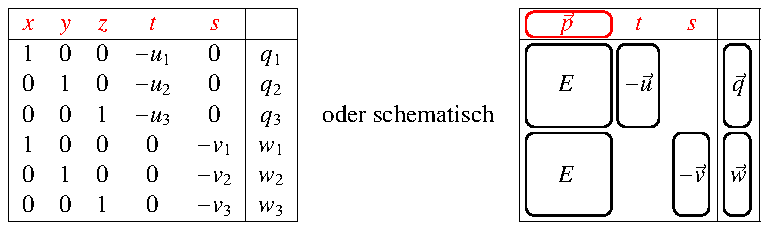
\includegraphics{3/images/schnittpunkttableau.pdf}
\label{skript:gerade:schnittpunkttableau}
\end{equation}
entspricht.
Eine einzige Durchführung des Gauss-Algorithmus wird alle verlangten Antworten
liefern.

\begin{beispiel}
Man finde den Schnittpunkt der Geraden $g_1$ und $g_2$ mit den
Parameterdarstellungen
\begin{align*}
g_1:
\vec r
&=t\begin{pmatrix}5\\6\\1\end{pmatrix}+\begin{pmatrix}0\\4\\2\end{pmatrix}
&
g_2:
\vec r
&=s\begin{pmatrix}5\\2\\4\end{pmatrix}+\begin{pmatrix}-15\\-6\\-7\end{pmatrix}
\end{align*}

\smallskip

%{\parindent 0pt Durch}
%Gleichsetzen erhält man ein Gleichungssystem mit drei Gleichungen
%für die zwei Unbekannten $s$ und $t$:
%\[
%t\begin{pmatrix}5\\6\\1\end{pmatrix}
%-s\begin{pmatrix}5\\2\\4\end{pmatrix}
%=\begin{pmatrix}-15\\-6\\-7\end{pmatrix}
%-\begin{pmatrix}0\\4\\2\end{pmatrix}
%=\begin{pmatrix}-15\\-10\\-9\end{pmatrix}
%\]
{\parindent 0pt Das}
Tableau \eqref{skript:gerade:schnittpunkttableau} für die Bestimmung
des Schnittpunktes ist
\begin{equation*}
\begin{tabular}{|>{$}c<{$}>{$}c<{$}>{$}c<{$}>{$}c<{$}>{$}c<{$}|>{$}c<{$}|}
\hline
\color{red}x&\color{red}y&\color{red}z&\color{red}t&\color{red}s&\\
\hline
1&0&0&-5& 0&0\\
0&1&0&-6& 0&4\\
0&0&1&-1& 0&2\\
1&0&0& 0&-5&-15\\
0&1&0& 0&-2&-6\\
0&0&1& 0&-4&-7\\
\hline
\end{tabular}
\qquad\rightarrow\qquad
\begin{tabular}{|>{$}c<{$}>{$}c<{$}>{$}c<{$}>{$}c<{$}>{$}c<{$}|>{$}c<{$}|}
\hline
\color{red}x&\color{red}y&\color{red}z&\color{red}t&\color{red}s&\\
\hline
1&0&0&0&0&-5\\
0&1&0&0&0&-2\\
0&0&1&0&0&1\\
0&0&0&1&0&-1\\
0&0&0&0&1&2\\
\hdashline
0&0&0&0&0&0\\
\hline
\end{tabular}
\end{equation*}
Die Null in der rechten unteren Ecke zeigt, dass sich die Geraden
tatsächlich schneiden.
In den Spalten für $t$ und $s$ lesen wir die Parameterwerte
$t=-1$ und $s=2$ ab,
und in den Spalten $x$, $y$ und $z$ die Koordinaten des
Schnittpunktes
$S=(-5,-2,1)$.
\end{beispiel}

Die schematische Darstellung 
\eqref{skript:gerade:schnittpunkttableau}
rechts zeigt, dass dieses Vorgehen für beliebige Dimension $n$
funktioniert auf ein Gleichungssystem mit $n+2$ Unbekannten und
$2n$ Gleichungen führt.
Im Falle $n=2$ hat man $4$ Gleichungen und $4$ Unbekannte.
Der Fall, dass die Gleichungen keine Lösungen haben ist immer noch
möglich, er tritt auf, wenn die beiden Geraden parallel sind.
Dies kann man wie folgt einsehen.
Führt man die ersten zwei Schritt der Vorwärtsreduktion durch
\[
\begin{tabular}{|>{$}c<{$}>{$}c<{$}>{$}c<{$}>{$}c<{$}|>{$}c<{$}|}
\hline
\color{red}x&\color{red}y&\color{red}t&\color{red}s&\\
\hline
1&0&-r_1&   0&p_1\\
0&1&-r_2&   0&p_2\\
1&0&   0&-v_1&q_1\\
0&1&   0&-v_2&q_2\\
\hline
\end{tabular}
\rightarrow
\begin{tabular}{|>{$}c<{$}>{$}c<{$}>{$}c<{$}>{$}c<{$}|>{$}c<{$}|}
\hline
\color{red}x&\color{red}y&\color{red}t&\color{red}s&\\
\hline
1&0&-r_1&   0&p_1\\
0&1&-r_2&   0&p_2\\
0&0& r_1&-v_1&q_1\\
0&1&   0&-v_2&q_2\\
\hline
\end{tabular}
\rightarrow
\begin{tabular}{|>{$}c<{$}>{$}c<{$}>{$}c<{$}>{$}c<{$}|>{$}c<{$}|}
\hline
\color{red}x&\color{red}y&\color{red}t&\color{red}s&\\
\hline
1&0&-r_1&   0&p_1\\
0&1&-r_2&   0&p_2\\
0&0& r_1&-v_1&q_1\\
0&0& r_2&-v_2&q_2\\
\hline
\end{tabular}
\]
Das Gleichungssystem ist genau dann nicht lösbar, wenn in dem kleineren
Tableau unten rechts keine Nullzeile auftritt.
Dies passiert genau dann, wenn die Vektoren $\vec{r}$ und $\vec{v}$ 
linear abhängig sind, wenn die Geraden also parallel sind.

%
% Gerade als Bild einer linearen Abbildung
%
\subsection{Gerade als Bild einer linearen Abbildung}
\begin{figure}
\centering
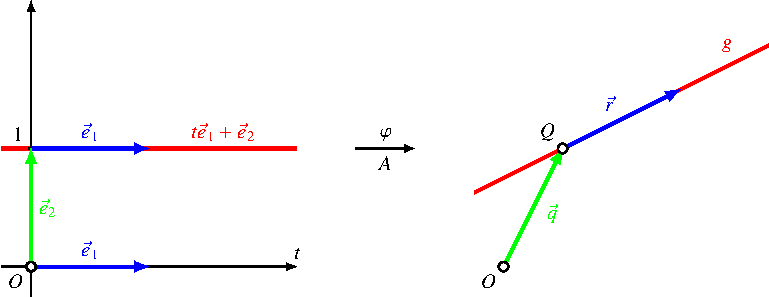
\includegraphics{3/images/geradeabb.pdf}
\caption{Gerade $g$ mit Parameterdarstellung $\vec{p} = t\vec{r}+\vec{q}$
als Bild einer Standardgeraden $\vec{p}=t\vec{e}_1+\vec{e}_2$ unter
einer linearen Abbildung, die $\vec{e}_1\mapsto\vec{r}$
und $\vec{e}_2\mapsto\vec{q}$ abbildet.
\label{skript:gerade:geradabb}}
\end{figure}
Eine lineare Abbildung ist gegeben durch die Bilder der
Standardbasisvektoren.
Sei die Gerade $g$ mit der Parameterdarstellung
\[
\vec{p}
=
\vec{q} + t\vec{r}
\]
gegeben.
Wir wählen die Vektoren $\vec{r}$ und $\vec{p}$ als Bilder der
Standardbasisvektoren der linearen Abbildung $\varphi$ ihre Matrix ist
daher 
\[
A=
\begin{pmatrix}
q_1   &r_1   \\
q_2   &r_2   \\
\vdots&\vdots\\
q_n   &r_n   
\end{pmatrix}.
\]
Die Abbildung bildet die Vektoren der roten Geraden in
Abbildung~\eqref{skript:gerade:geradabb} links auf die Punkte der
Geraden $g$ in der Abbildung rechts ab:
\[
\varphi
:
\begin{pmatrix}
t\\1
\end{pmatrix}
\mapsto
\vec{q}+t\vec{r}.
\]
Wir lernen zwei Dinge aus dieser Beobachtung:
\begin{enumerate}
\item
Jede Gerade ist Bild der selben Gerade.
Man könnte also auch sagen, dass die affine Geometrie der Geraden
die Geometrie der möglichen linearen Abbildungen der Ebene ist.
Aus dieser Perspektive muss man vor allem lernen, mit linearen
Abbildungen zu arbeiten.
\item
Eine lineare Abbildung bildet den Nullpunkt wieder auf den Nullpunkt ab.
Die Verwendung einer zusätzlichen zweiten Koordinate, die immer den
Wert $1$ hat, ermöglicht uns, eine Verschiebungen hinzuzufügen.
Diese Idee der homogenen Koordinaten wird in Abschnitt~\ref{section:kamera}
bei der Diskussion der Abbildung durch eine Kamera eine wesentliche Rolle
spielen.
\end{enumerate}


%
%
%
\subsection{Gerade in der Ebene als Nullmenge}
Eine einzelne lineare Gleichung der Form 
\[
ax+by=c
\]
kann mit dem Gauss-Algorithmus
\[
\begin{tabular}{|>{$}c<{$} >{$}c<{$}|>{$}c<{$}|}
\hline
x&y&\\
\hline
a&b&c\\
\hline
\end{tabular}
\quad\rightarrow\quad
{
\def\arraystretch{1.2}
\begin{tabular}{|>{$}c<{$} >{$}c<{$}|>{$}c<{$}|}
\hline
x&y&\\
\hline
1&\frac{b}{a}&\frac{c}{a}\\
\hline
\end{tabular}
}
\]
Daraus liest man die Lösungsmenge
\[
\mathbb L
=
\left\{
\left.
\begin{pmatrix} x\\ y \end{pmatrix}
=
\begin{pmatrix} \frac{c}{a}\\0 \end{pmatrix}
+
y\begin{pmatrix} -\frac{b}{a} \\ 1 \end{pmatrix}
\right|
\;
y\in\mathbb R
\right\}.
\]
In der Mengenklammer steht aber gerade die Parameterdarstellung
einer Gerade mit dem Parameter $y$.

Umgekehrt kann man zu jeder Parameterdarstellung
$
\vec{p} + t\vec{r}
$
einer Geraden
in der Ebene eine lineare Gleichung angeben.
Dazu muss man die Konstanten $a$, $b$ und $c$ so bestimmen,
dass die Gleichung zum Beispiel für den Stützvektor $\vec{p}$ und 
für den Punkt $\vec{p}+\vec{r}$ erfüllt ist.
Indem man die Koordinaten dieser Punkte einsetzt, erhält man
zwei Gleichungen
\[
\begin{linsys}{2}
p_1 a&+&p_2b&=&c\\
(p_1+q_1)a&+&(p_2+q_2)b&=&c
\end{linsys}
\]
für die drei Unbekannten $a$, $b$ und $c$.
In ein Tableau übertragen
\[
\begin{tabular}{|>{$}c<{$}>{$}c<{$}>{$}c<{$}|>{$}c<{$}|}
\hline
a&b&c&\\
\hline
p_1 & p_2 & -1&0\\
p_1+q_1&p_2+q_1&-1&0\\
\hline
\end{tabular}
\rightarrow
\begin{tabular}{|>{$}c<{$}>{$}c<{$}>{$}c<{$}|>{$}c<{$}|}
\hline
a&b&c&\\
\hline
p_1&p_2&-1&0\\
q_1&q_2&0&0\\
\hline
\end{tabular}
\rightarrow
\begin{tabular}{|>{$}c<{$}>{$}c<{$}>{$}c<{$}|>{$}c<{$}|}
\hline
a&b&c&\\
\hline
1&0&u_1&0\\
0&1&u_2&0\\
\hline
\end{tabular}
\]
Daraus liest man ab, dass $c$ eine frei wählbare Variable ist und dass
man $a=u_1c$ und $b=u_2c$ verwenden muss.

\begin{beispiel}
Man finde eine lineare Gleichung, deren Lösungsmenge die Gerade mit
Parameterdarstellung
\[
\begin{pmatrix} 1\\2\end{pmatrix} + t\begin{pmatrix}2\\1\end{pmatrix}
\]
ist.
\smallskip

Wir müssen das Gleichungssystem
\[
\begin{tabular}{|>{$}c<{$}>{$}c<{$}>{$}c<{$}|>{$}c<{$}|}
\hline
a&b&c&\\
\hline
1&2&-1&0\\
2&1&0&0\\
\hline
\end{tabular}
\rightarrow
\begin{tabular}{|>{$}c<{$}>{$}c<{$}>{$}c<{$}|>{$}c<{$}|}
\hline
a&b&c&\\
\hline
1&0& \frac13&0\\
0&1&-\frac23&0\\
\hline
\end{tabular}
\]
Daraus lesen wir ab, dass wir mit $c=3$ die Gleichung mit $a=-1$ und $b=2$
verwenden können, also
\[
-x+2y=3.
\]
Durch Einsetzen der Punkte $(1,2)$ und $(3,3)$ kann man sich überzeugen,
dass die Lösungsmenge dieser Gleichung mit der Geraden zusammenfällt.
\qedhere
\end{beispiel}

%
% Parallele Geraden
%
\subsection{Parallele Geraden}
Wie kann man herausfinden, ob zwei Geraden in der Ebene parallel sind?

\begin{aufgabe}
Gegeben zwei Geraden in Parameterdarstellung
\[
\vec{r} = \vec{p} + t\vec{r}
\qquad\text{und}\qquad
\vec{r} = \vec{q} + t\vec{v},
\]
entscheide, ob die Geraden parallel sind.
\end{aufgabe}
Die Geraden sind parallel, wenn sie keine Schnittpunkte haben, oder
wenn das Gleichungssystem
\[
\vec{p} + t\vec{r}
=
\vec{q} + s\vec{v}
\qquad\Leftrightarrow\qquad
t\vec{r}
-
s\vec{v}
=
\vec{q}
-
\vec{p}
\]
keine Lösung hat.
Dies ist ein Gleichungssystem mit zwei Gleichungen für zwe Unbekannte.
Es kann nur im singulären Fall keine Lösung haben.
Dieser tritt ein, wenn die Vektoren $\vec{r}$ und $\vec{v}$
linear abhängig sind.
Dieses Kriterium funktioniert aber auch im Raum: zwei Geraden sind
genau dann parallel, wenn die Richtungsvektoren linear abhängig sind.

